% file: counting-sort-cycle.tex

\documentclass[tikz]{standalone}
\usetikzlibrary{shapes, chains, positioning, arrows.meta, shapes.multipart}

\newcommand{\red}[1]{\textcolor{red}{#1}}
\newcommand{\blue}[1]{\textcolor{blue}{#1}}
\newcommand{\purple}[1]{\textcolor{purple}{#1}}

\begin{document}
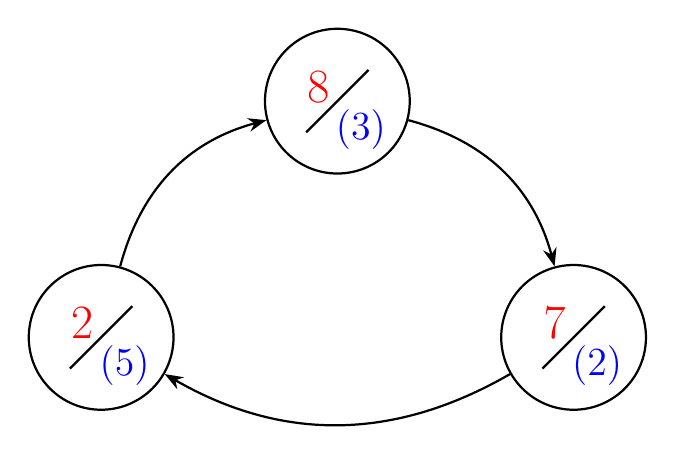
\begin{tikzpicture}[]
  \def \radius {3cm}

  \foreach \s/\pos/\index/\ele in {1/90/8/3, 2/0/7/2, 3/-180/2/5} {
    \node[circle solidus, draw, thick, inner sep = 1pt] (\s) at (\pos:\radius) {
      \red{\LARGE $\index$} \nodepart{lower} \blue{\Large $(\ele)$}
    };
  }

  \path[draw, ->, >=Stealth, thick, every edge/.style = {bend left, draw}]
      (1) edge (2)
      (2) edge (3)
      (3) edge (1);
\end{tikzpicture}
\end{document}
